% AER E 361 Mission Report Template
% Spring 2023
% Template created by Yiqi Liang and Professor Matthew Nelson

% Document Configuration DO NOT CHANGE
\documentclass[12 pt]{report}
% --------------------LaTeX Packages---------------------------------
% The following are packages that are used in this report.
% DO NOT CHANGE ANY OF THE FOLLOWING OR YOUR REPORT WILL NOT COMPILE
% -------------------------------------------------------------------

\usepackage{hyperref}
\usepackage{parskip}
\usepackage{titlesec}
\usepackage{titling}
\usepackage{graphicx}
\usepackage{graphviz}
\usepackage[T1]{fontenc}
\usepackage{titlesec, blindtext, color} %for LessIsMore style
\usepackage{tcolorbox} %for references box
\usepackage[hmargin=1in,vmargin=1in]{geometry} % use 1 inch margins
\usepackage{float}
\usepackage{tikz}
\usepackage{svg} % Allows for SVG Vector graphics
\usepackage{textcomp, gensymb} %for degree symbol
\hypersetup{
	colorlinks=true,
	linkcolor=blue,
	urlcolor=cyan,
}
\usepackage{biblatex}
\addbibresource{main.bib}
\usepackage{amsmath}
\usepackage{listings}
\usepackage{multicol}
\usepackage{array}

\usepackage{hologo} %KYR: for \BibTeX
%\usepackage{algpseudocode}
%\usepackage{algorithm}
% This configures items for code listings in the document
\usepackage{xcolor}

\usepackage{fancyhdr} % Headers/Footers
\usepackage{siunitx} % SI units
\usepackage{csquotes} % Display Quote
\usepackage{microtype} % Better line breaks

% The following package and lines define a special type of list
\usepackage{enumitem}
\newlist{parlist}{enumerate}{2}
\setlist[parlist, 1]{label=(\roman*),wide=0pt,topsep=0pt,labelindent=20pt,leftmargin=20pt}

\definecolor{commentsColor}{rgb}{0.497495, 0.497587, 0.497464}
\definecolor{keywordsColor}{rgb}{0.000000, 0.000000, 0.635294}
\definecolor{stringColor}{rgb}{0.558215, 0.000000, 0.135316}
\definecolor{mygreen}{rgb}{0,0.6,0}
\definecolor{mygray}{rgb}{0.5,0.5,0.5}
\definecolor{mymauve}{rgb}{0.58,0,0.82}

\lstdefinestyle{customc}{
  belowcaptionskip=1\baselineskip,
  breaklines=true,
  frame=L,
  xleftmargin=\parindent,
  language=C,
  showstringspaces=false,
  basicstyle=\footnotesize\ttfamily,
  keywordstyle=\bfseries\color{green!40!black},
  commentstyle=\itshape\color{purple!40!black},
  identifierstyle=\color{blue},
  stringstyle=\color{orange},
 }

 \lstset{ %
  backgroundcolor=\color{white},   % choose the background color; you must add \usepackage{color} or \usepackage{xcolor}
  basicstyle=\footnotesize,        % the size of the fonts that are used for the code
  breakatwhitespace=false,         % sets if automatic breaks should only happen at whitespace
  breaklines=true,                 % sets automatic line breaking
  captionpos=b,                    % sets the caption-position to bottom
  commentstyle=\color{commentsColor}\textit,    % comment style
  deletekeywords={...},            % if you want to delete keywords from the given language
  escapeinside={\%*}{*)},          % if you want to add LaTeX within your code
  extendedchars=true,              % lets you use non-ASCII characters; for 8-bits encodings only, does not work with UTF-8
  frame=tb,	                   	   % adds a frame around the code
  keepspaces=true,                 % keeps spaces in text, useful for keeping indentation of code (possibly needs columns=flexible)
  keywordstyle=\color{keywordsColor}\bfseries,       % keyword style
  language=Python,                 % the language of the code (can be overrided per snippet)
  otherkeywords={*,...},           % if you want to add more keywords to the set
  numbers=left,                    % where to put the line-numbers; possible values are (none, left, right)
  numbersep=8pt,                   % how far the line-numbers are from the code
  numberstyle=\tiny\color{commentsColor}, % the style that is used for the line-numbers
  rulecolor=\color{black},         % if not set, the frame-color may be changed on line-breaks within not-black text (e.g. comments (green here))
  showspaces=false,                % show spaces everywhere adding particular underscores; it overrides 'showstringspaces'
  showstringspaces=false,          % underline spaces within strings only
  showtabs=false,                  % show tabs within strings adding particular underscores
  stepnumber=1,                    % the step between two line-numbers. If it's 1, each line will be numbered
  stringstyle=\color{stringColor}, % string literal style
  tabsize=2,	                   % sets default tabsize to 2 spaces
  title=\lstname,                  % show the filename of files included with \lstinputlisting; also try caption instead of title
  columns=fixed                   % Using fixed column width (for e.g. nice alignment)
}

\lstdefinestyle{customasm}{
  belowcaptionskip=1\baselineskip,
  frame=L,
  xleftmargin=\parindent,
  language=[x86masm]Assembler,
  basicstyle=\footnotesize\ttfamily,
  commentstyle=\itshape\color{purple!40!black},
}

\lstset{escapechar=@,style=customc}

\titlelabel{\thetitle.\quad}

% From here on out you can start editing your document
\newcommand{\subtitle}[1]{%
  \posttitle{%
    \par\end{center}
    \begin{center}\LARGE#1\end{center}
    \vskip0.5em}%
}

\title{\textbf{Iowa State University
\\{\Large Aerospace Engineering}}}
\subtitle{AER E 322 Lab 4\\
		  Strain Gage Application and Testing}
\author{Matthew Mehrtens, Peter Mikolitis, and Natsuki Oda}

\newcommand{\etal}{\textit{et al}., }
\newcommand{\ie}{\textit{i}.\textit{e}., }
\newcommand{\eg}{\textit{e}.\textit{g}., }

% Define the headers and footers
\setlength{\headheight}{70.63135pt}
\geometry{head=70.63135pt, includehead=true, includefoot=true}
\fancypagestyle{plain}{
	\fancyhead{}\fancyfoot{} % clears the headers/footers
	\fancyhead[L]{\textbf{AER E 322}}
	\fancyhead[C]{\textbf{Aerospace Structures Laboratory Report}\\
					 \textbf{Lab 4 Strain Gage Application and Testing}\\
					 Section 4 Group 2\\
					 Matthew Mehrtens, Peter Mikolitis, and Natsuki Oda\\
					 \today}
	\fancyhead[R]{\textbf{Spring 2023}}
	\fancyfoot[C]{\thepage}
}
\pagestyle{fancy}
\fancyhead{}\fancyfoot{} % clears the headers/footers
\fancyhead[L]{\textbf{AER E 322}}
\fancyhead[C]{\textbf{Aerospace Structures Laboratory Report}\\
			  \textbf{Lab 4 Strain Gage Application and Testing}\\
			  Section 4 Group 2\\
			  Matthew Mehrtens, Peter Mikolitis, and Natsuki Oda\\
			  \today}
\fancyhead[R]{\textbf{Spring 2023}}
\fancyfoot[C]{\thepage}

\begin{document}
\maketitle
\tableofcontents

\chapter{Pre-Lab} \label{ch:pre-lab}
\section{Introduction} \label{sec:introduction}
In this lab, our group was tasked with attaching a strain gauge to the surface of an aluminum part, then testing the part under bending and tensile loads. We first attached the strain gauge to the part's surface according to the directions provided, then soldered lead wires to the gauge so it could be tested using a Vishay P-3500. The tensile load test will occur once and be calibrated using data collected from testing a steel plate. The bending test will have multiple trials that will be averaged to get a final value.

\section{Objectives} \label{sec:objectives}
\begin{itemize}
	\item Learn how to attach a strain gauge to the surface of a part 
	\item Collect usable data from both the bending test and tensile test 
	\item Learn how to work with the Vishay P-3500 
\end{itemize}

\section{Hypothesis} \label{sec:hypothesis}
\begin{itemize}
	\item For the bending test, we expect a much more substantial readout while bending it versus putting the specimen in tension by hand.
	\item We expect a much greater strain readout for the tensile test while applying tension than bending it.
	\item The bending test will have more accurate data because multiple trials are averaged, whereas the tensile test only occurs once. For this reason, we expect the bending data to be much more accurate than tensile testing.
\end{itemize} 

\chapter{Lab Work} \label{ch:lab_work}
\section{Work Assignments} \label{sec:work_assignments}
Refer to Table \ref{fig:work_assignments} for the distribution of work during this lab.

\begin{table}[!htbp]
\caption{Work assignments for AER E 322 Lab <lab number>.}
\begin{center}
	\begin{tabular}{| c | c | c | c |}
		\hline
		\multicolumn{1}{| c |}{\textbf{Task}}&\textbf{Matthew}&\textbf{Peter}&\textbf{Natsuki}\\
		\hline
		\multicolumn{4}{| c |}{\textit{Lab Work}}\\
		\hline
		Date Recording&X&&\\
		\hline
		Exp. Setup&X&X&X\\
		\hline
		Exp. Work&X&X&X\\
		\hline
		Exp. Clean-Up&X&X&X\\
		\hline
		\multicolumn{4}{| c |}{\textit{Post Lab}}\\
		\hline
		Data Analysis&X&X&\\
		\hline
		\multicolumn{4}{| c |}{\textit{Report}}\\
		\hline
		Introduction&&X&\\
		\hline
		Objectives&X&&X\\
		\hline
		Hypothesis&X&&\\
		\hline
		Variables&X& & \\
		\hline
		Materials&&&X\\
		\hline
		Apparatus&X&&\\
		\hline
		Procedures&&&X\\
		\hline
		Data&X&X&X\\
		\hline
		Analysis&X&X&X\\
		\hline
		Conclusion&&X&\\
		\hline
		References&X&&\\
		\hline
		Appendix&X&&\\
		\hline
		Revisions&X&X&\\
		\hline
		Editing&X&&\\
		\hline
	\end{tabular}
\end{center}
\label{fig:work_assignments}
\end{table}

\section{Materials} \label{sec:materials}
Materials required for the specimen:
\begin{itemize}
	\item SGD-5/350-LY13 strain gages
	\item 2024-O Alumninum alloy plate
	\item Acetone for cleaning surface of specimen
	\item Clear tape
	\item Sanding paper
	\item 496 bonder
	\item solder
\end{itemize}

Materials required for the tests:
\begin{itemize}
	\item The Vishay P-3500 strain indicator
	\item Steel plate for calibration
	\item Instron load frame stration
\end{itemize}

\section{Apparatus} \label{sec:apparatus}
The specimen is an aluminum alloy plate with strain gages attached on each side. Gages are attached to the aluminum plate with clear tape and glue. Strain gages are connected to the yellow readout box through wires, and the wire of the gages and readout box are connected by soldering. In the bending test, each end of the specimen is set onto the stable tables. And the load is applied on the center of the specimen by putting mass on. In a tensile test, the specimen is set into an Instron load flame station with the correct fastened position. These apparatuses are shown in Figures \ref{fig:bending_pic} and \ref{fig:tensile_pic}

\begin{figure}[htbp]
	\centering
	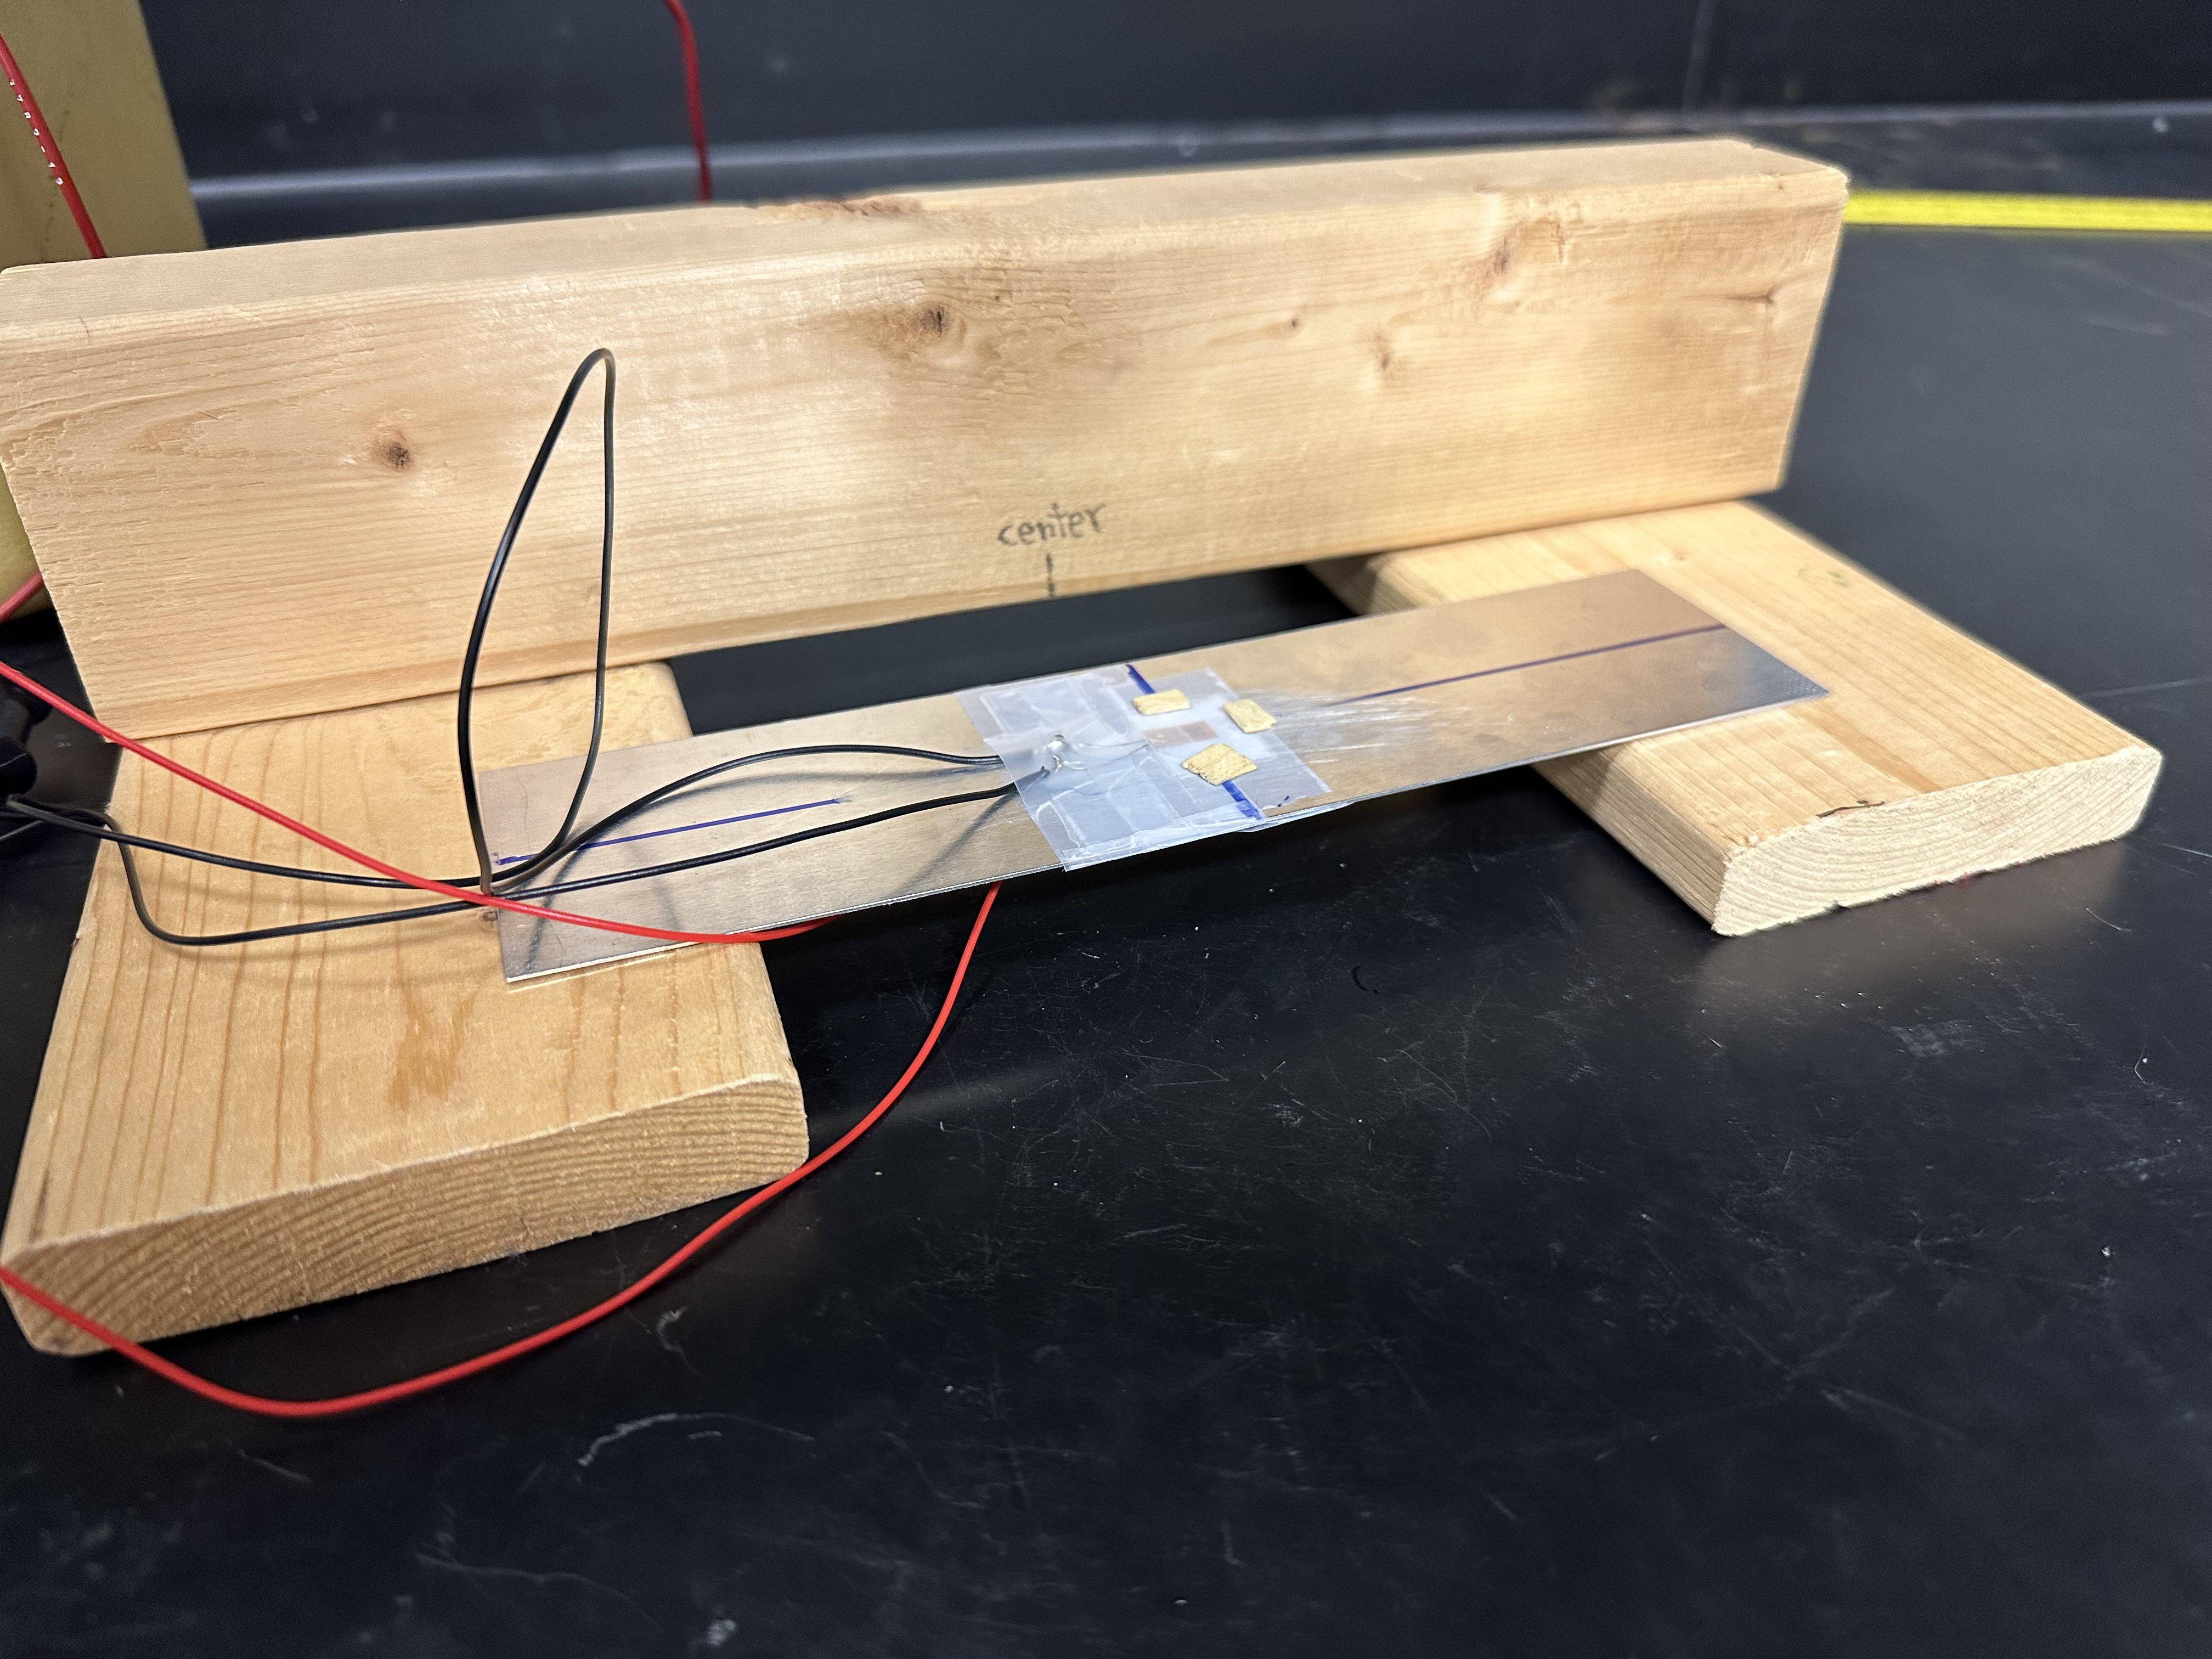
\includegraphics[width=4in]{images/IMG_1074}
	\caption{The bending test apparatus.}
	\label{fig:bending_pic}
\end{figure}

\begin{figure}[htbp]
	\centering
	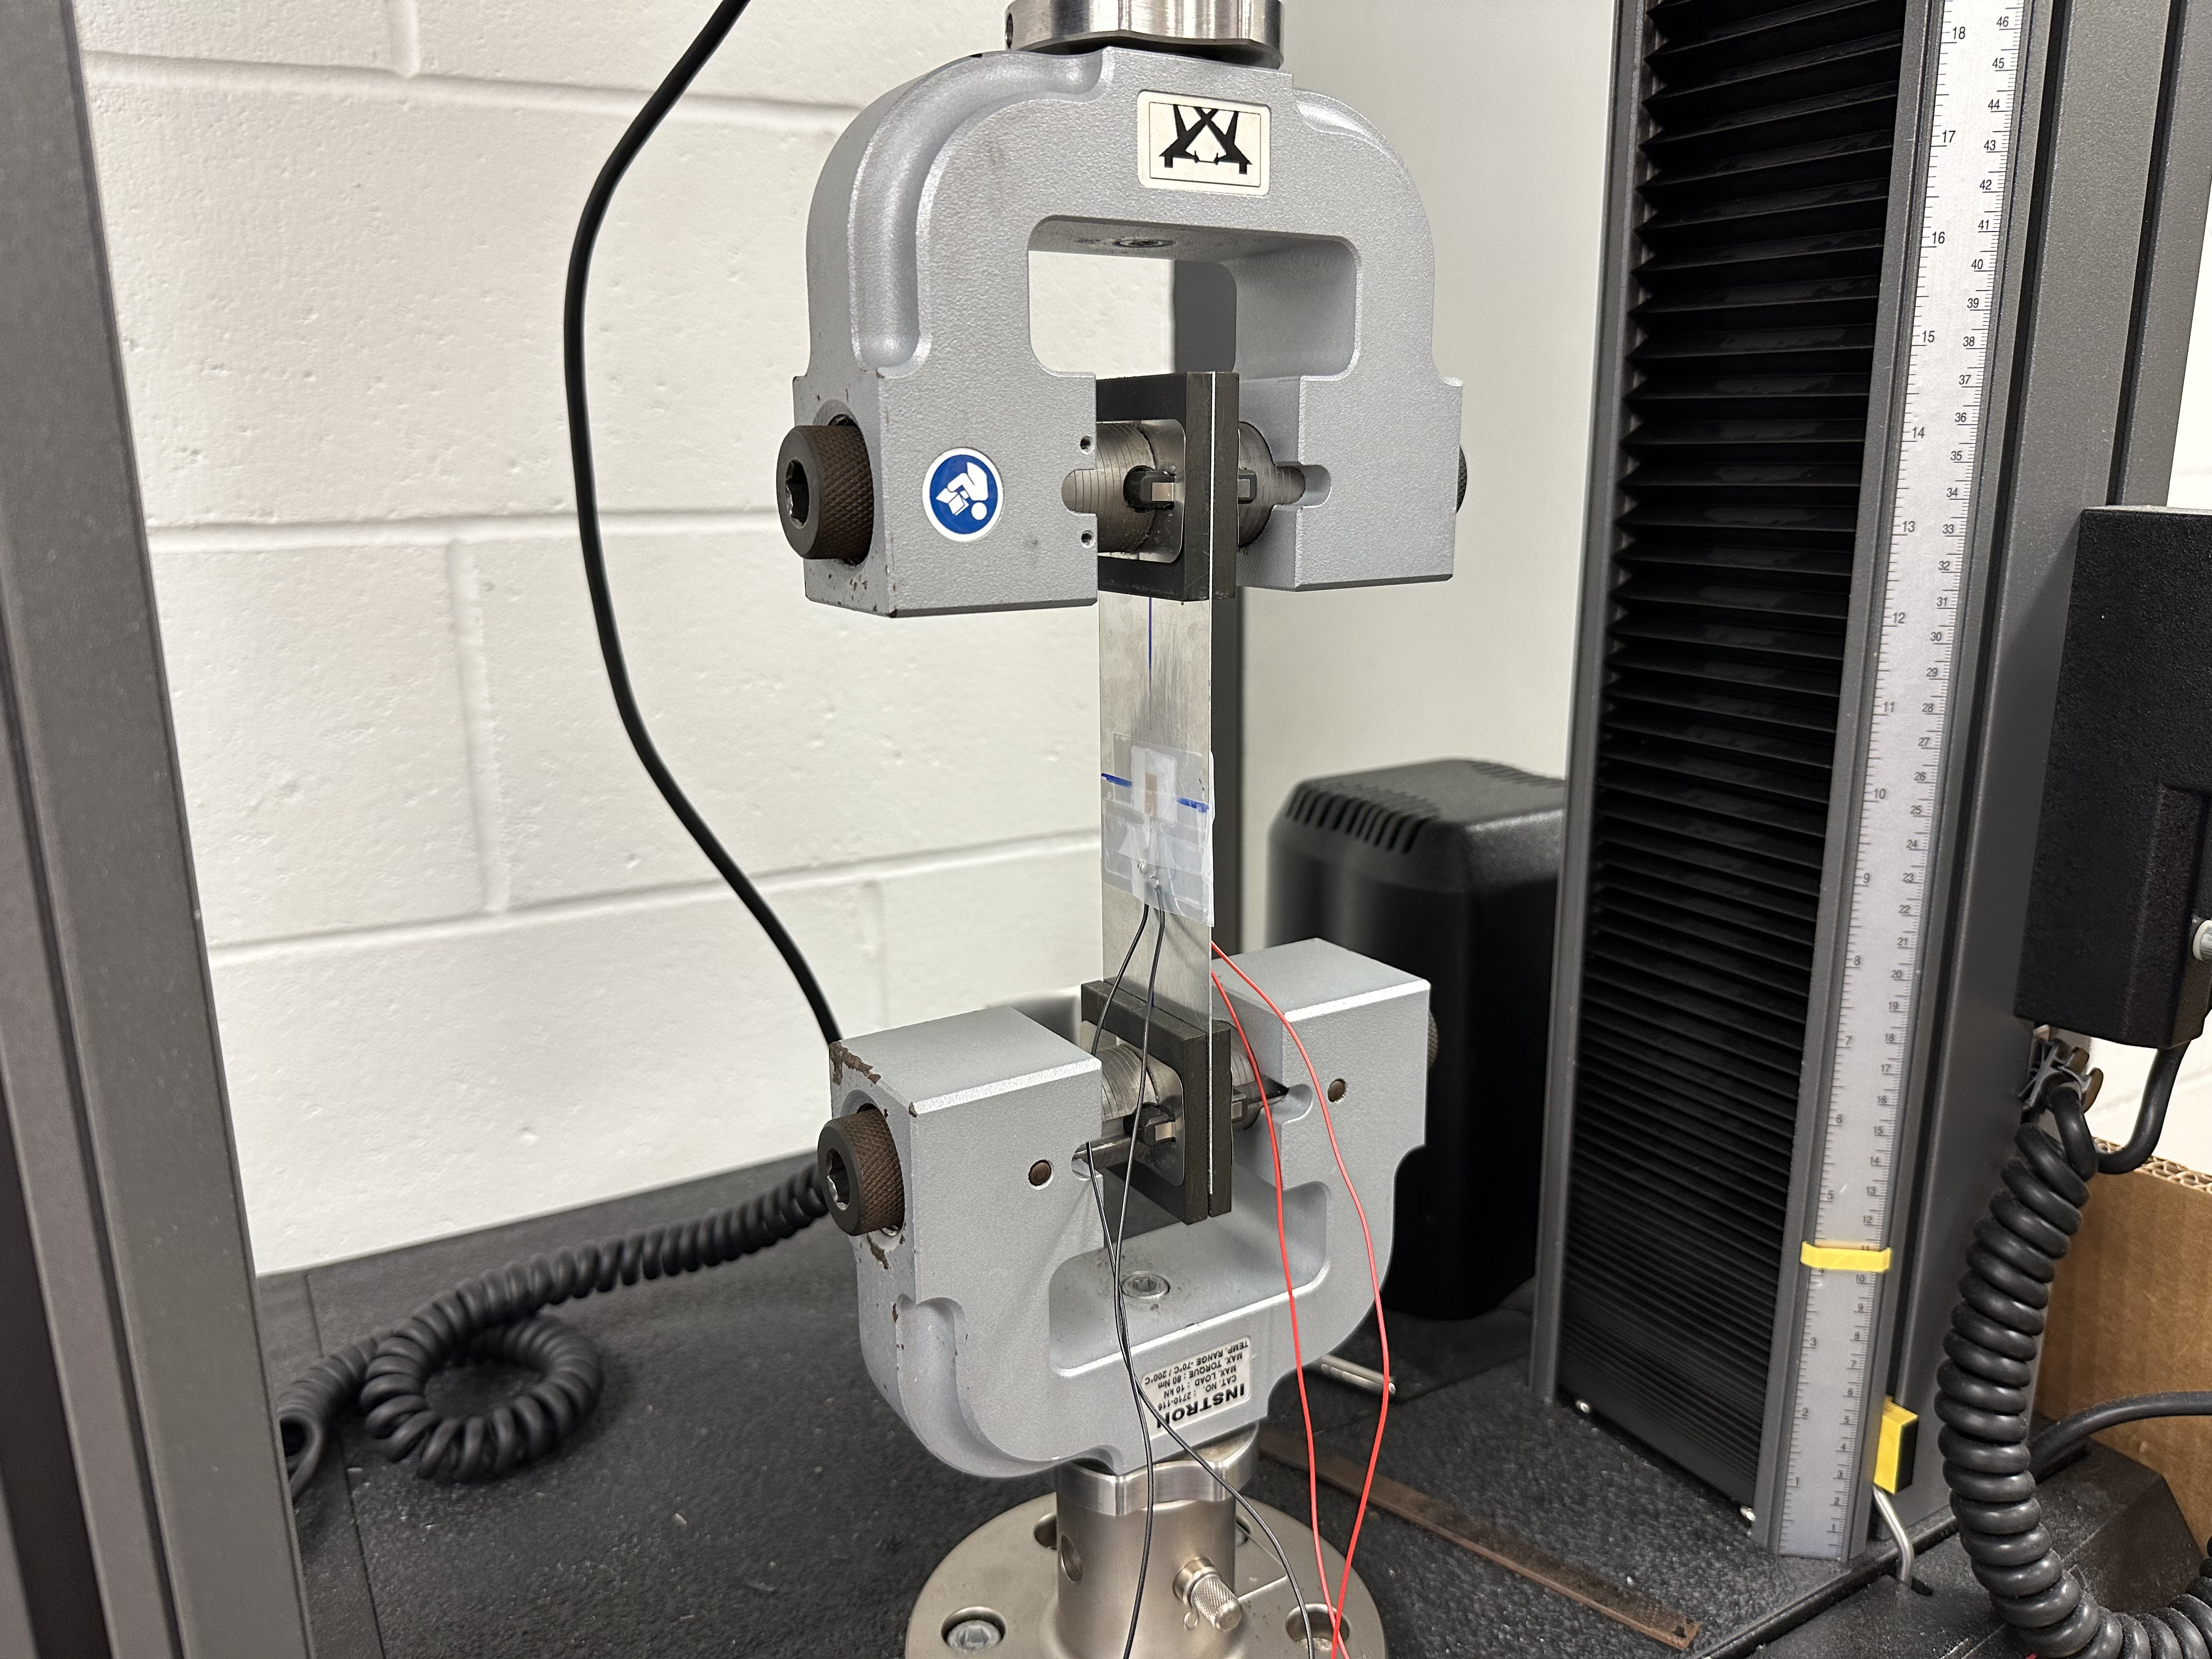
\includegraphics[width=4in]{images/IMG_1073}
	\caption{The tensile test apparatus.}
	\label{fig:tensile_pic}
\end{figure}

\section{Procedures} \label{sec:procedures}
First, to prepare the specimen, measure the center points on each side where strain gages are applied, then clear the surface of each aluminum plate side by sanding paper and acetone. To tape strain gages onto the center of the plate, hold each end of the clear tape while orienting the long side of the tape perpendicular to the long side of the specimen. Attach the tape with a strain gauge onto the center position of aluminum plates lightly, and then apply a small drop of glue between the plate and a gauge. And then, keep attaching strain gages on the plate by fingers for about two minutes. Remove the tape after confirming strain gages are completely stuck on the plate with glue, and tape under the lead wires for insulation. To connect wires with strain gages, strip wires about one inch from all ends. Make a knot between wires and those from strain gages, and do soldering onto the knots. This must be done in all knots. After finishing soldering and removing residues, confirm whether all wires are connected to strain gages using Voltmeter. When wires are connected correctly, the resistance readout will be between one and two ohms.      

Connect strain gages and yellow readout box through test clips for bending test preparation. Set both ends of the specimen onto a stable table. Measure the length between the top side of the specimen and the ground and the distance between both ends of the specimen. After setting up everything, check if a substantial change happens by pushing the center of the specimen. Find where the load is applied. This position needs to be close to a strain gauge. After checking the position, put two spacers on. Before applying load, ensure that the parameter shown on the readout box is zero each time. If not, set the parameter to zero by turning the balance knob. Put a mass after checking the readout, and measure the length between the ground and top side of the aluminum plate with a ruler and the readout value on the readout yellow box. Also, measure the length between the ground and the top side of the specimen again after removing the mass. This process should be done several times. Take averages of the readouts. 

Before the tensile test, conduct calibration to measure system error. First, set a steel plate into an Instron load flame with each end of the specimen fastened well. Make sure that the calibration plate is parallel to the Instron load flame. After setting the plate up, apply load with \qty{0.00061}{in} elongation and by approximately \qty{80}{lbf} after the value of setting load and extension as zero. Record extension and load value each time a constant load is applied. This process continues until the load reaches \qty{400}{lbs} after calibration. Set the specimen with the same method as the calibration plate and connect the specimen to the yellow readout box. Open the software, BlueHill3 for recording data and for controlling to apply load. Save the test file with the team name and the team’s section. Activate the strain vs. time recording and make graphs from strain gages and Instron load flame visible on the desktop screen. Set and make sure the value of extension and load are zero. Push the start button to activate strain gages, and immediately push the start button to start a tensile test. Push both finish buttons immediately after \qty{50}{s} pass, and the load reaches \qty{300}{lbs}. At last, save the collected data. 

\section{Data} \label{sec:data}
Our collected data is shown in Figure \ref{fig:data} with more data shown in Section \ref{sec:analysis}.

\begin{figure}[htbp]
	\centering
	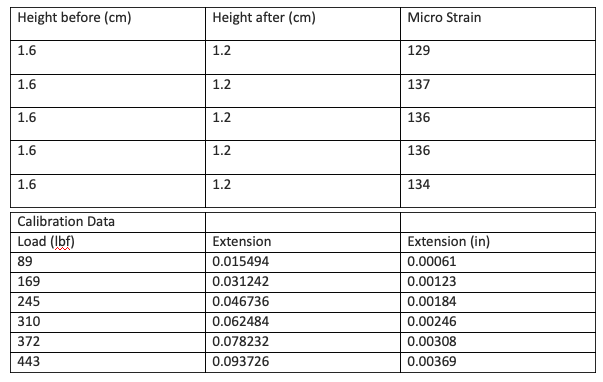
\includegraphics[width=4in]{images/Data}
	\caption{The bending test and calibration data.}
	\label{fig:data}
\end{figure}

\chapter{Conclusion} \label{ch:conclusion}
\section{Analysis} \label{sec:analysis}
\begin{parlist}
	\item When the sample was configured for the bending test, we were unable to produce any substantial change when pulling the specimen in tension. This is expected, and we can demonstrate it theoretically. We begin by first referring to the Wheatstone Bridge Equation, Equation \ref{eqn:wheatstone_eqn}, on page five of the lecture slides \cite{slides}.
	\begin{align} \label{eqn:wheatstone_eqn}
		\frac{V}{E}&=\frac{R_3}{R_3+R_4	}-\frac{R_1}{R_1+R_2}
	\end{align}
	One page \num{14}, a relationship is given between $\frac{V}{E}$ and $\varepsilon$, as shown in Equation \ref{eqn:wheatstone_wrt_strain}.
	\begin{align} \label{eqn:wheatstone_wrt_strain}
		\frac{V}{E}&=\beta{}GF\varepsilon
	\end{align}
	From Equation \ref{eqn:wheatstone_wrt_strain}, it is obvious that if $\frac{V}{E}$ is zero, then the strain, $\varepsilon$, will also be zero.
	
	For the bending test, the NI USB-6000 was set to a Half Bridge I Wheatstone configuration. For a small deflection in the sample, resulting in a change in resistance of $\Delta{}R$, these are the typical equations for $R_1$--$R_4$:
	\begin{align*}
		R_1&=R\\
		R_2&=R\\
		R_3&=R+{\Delta}R\\
		R_4&=R-{\Delta}R
	\end{align*}
	In this example, the sample is being pulled in tension rather than bent; so, we have
	\begin{align*}
		R_1&=R\\
		R_2&=R\\
		R_3&=R+\Delta{}R\\
		R_4&=R+\Delta{}R
	\end{align*}
	Plugging these values into Equation \ref{eqn:wheatstone_eqn}, we derive the following:
	\begin{align*}
		\frac{V}{E}&=\frac{R+\Delta{}R}{(R+\Delta{}R)+(R+\Delta{}R)}-\frac{R}{R+R}\\
		&=\frac{R+\Delta{}R}{2(R+\Delta{}R)}-\frac{R}{2R}\\
		&=\frac{1}{2}-\frac{1}{2}\\
		&=0
	\end{align*}
	Since $\frac{V}{E}=0$, we expect no change in $\varepsilon$ when pure tension is applied in the Half Bridge I Wheatstone configuration.
	
	\item When the sample was configured for the tensile test, we were unable to produce any substantial change when bending the specimen. This is expected, and we can demonstrate it theoretically. Again, we start by referring to \ref{eqn:wheatstone_eqn} and noting that when $\frac{V}{E}=0$, the strain, $\varepsilon$, will also be zero.
	
	For the tensile test, the NI USB-6000 was set to a Half Bridge II Wheatstone configuration. For a small deflection in the sample, resulting in a change in resistance of $\Delta{}R$, these are the typical equations for $R_1$--$R_4$:
	\begin{align*}
		R_1&=R\\
		R_2&=R+\Delta{}R\\
		R_3&=R+\Delta{}R\\
		R_4&=R
	\end{align*}
	In this example, the sample is being bent rather than pulled in tension; so, we have
	\begin{align*}
		R_1&=R\\
		R_2&=R+\Delta{}R\\
		R_3&=R-\Delta{}R\\
		R_4&=R
	\end{align*}
	Plugging these values into Equation \ref{eqn:wheatstone_eqn}, we derive the following:
	\begin{align*}
		\frac{V}{E}&=\frac{R-\Delta{}R}{(R-\Delta{}R)+R}-\frac{R}{R+(R+\Delta{}R)}
		&=\frac{R-\Delta{}R}{2R-\Delta{}R}-\frac{R}{2R+\Delta{}R}
	\end{align*}
	By the binomial theorem, we know
	\begin{align*}
		(2R+(-\Delta{}R))^{-1}&=(2R)^{-1}+(-1)(2R)^{-2}(-\Delta{}R)+\cdots\\
		&=(2R)^{-1}+(2R)^{-2}\Delta{}R+\cdots
	\end{align*}
	and
	\begin{align*}
		(2R+\Delta{}R)^{-1}&=(2R)^{-1}+(-1)(2R)^{-2}\Delta{}R+\cdots\\
		&=(2R)^{=1}-(2R)^{-2}\Delta{}R+\cdots
	\end{align*}
	With these two expansions, and disregarding all terms after those shown above, we continue with the derivation.
	\begin{align*}
		\frac{V}{E}&=(R-\Delta{}R)[(2R)^{-1}+(2R)^{-2}\Delta{}R+\cdots]-R[(2R)^{-1}-(2R)^{-2}\Delta{}R+\cdots]\\
		&=\frac{R-\Delta{}R}{2R}+\frac{\Delta{}R(R-\Delta{}R)}{4R^2}-\frac{1}{2}+\frac{\Delta{}R}{4R}\\
		&=\frac{R\Delta{}R}{4R^2}-\frac{\Delta{}R^2}{4R^2}+\frac{2(R-\Delta{}R)+\Delta{}R}{4R}-\frac{1}{2}\\
		&=\frac{\Delta{}R}{4R}-\frac{\Delta{}R^2}{4R^2}+\frac{2R-\Delta{}R}{4R}-\frac{1}{2}\\
		&=\frac{\Delta{}R}{4R}+\frac{1}{2}-\frac{\Delta{}R}{4R}-\frac{1}{2}-\frac{\Delta{}R^2}{4R^2}\\
		&=-\frac{\Delta{}R^2}{4R^2}
		&\approx0
	\end{align*}
	In the final step of the derivation, we assume that $\Delta{}R^2\approx0$ for small deflections. Furthermore, since $\frac{V}{E}\approx0$, we expect no significant change in $\varepsilon$ when pure bending is applied in the Half Bridge II Wheatstone configuration.
	
	\item To determine how close our actual strain measurements were to the theoretical values, we first must derive an equation that relates strain, $\varepsilon$, to the maximum deflection, $\nu_{max}$. We recall the following equations from mechanics:
	\begin{align} \label{eqn:nu_max}
		\nu_{max}&=\frac{PL^3}{48EI}
	\end{align}
	\begin{align} \label{eqn:bending_stress}
		\sigma&=\frac{My}{I}
	\end{align}
	\begin{align} \label{eqn:sigma_E_epsilon}
		\sigma&=E\varepsilon
	\end{align}
	We define $L$ to be the length between the two supports of the three-point bending test, $h$ to be the thickness of the sample, $b$ to be the width of the sample, and $P$ to be the load applied to the sample. We first make a theoretical cut at a distance of $\frac{L}{2}$ in the sample and calculate the sum of moments at that point, point $O$.
	\begin{align*}
		\sum{}M_O&=0\\
		M-\frac{P}{2}(\frac{L}{2})&=0\\
		M&=\frac{PL}{4}
	\end{align*}
	Substituting this moment equation into Equation \ref{eqn:bending_stress} we find
	\begin{align*}
		\sigma_{max}&=\frac{\frac{PL}{4}\frac{h}{2}}{I}\\
		&=\frac{PLh}{8I}
	\end{align*}
	Plugging the expression for $\sigma	_{max}$ into Equation \ref{eqn:sigma_E_epsilon}
	\begin{align*}
		\varepsilon&=\frac{PLh}{8EI}
	\end{align*}
	This expression can be further rearranged as follows
	\begin{align*}
		\frac{\varepsilon{}L^2}{6h}&=\frac{PL^3}{48EI}
	\end{align*}
	Since the RHS of this equation is equivalent to $\nu_{max}$, we substitute $\nu{max}$ for the RHS of this equation and solve for $\varepsilon$.
	\begin{align*}
		\frac{\varepsilon{}L^2}{6h}&=\nu_{max}\\
		\varepsilon&=\frac{6h\nu_{max}}{L^2}
	\end{align*}
	Plugging in the actual values, including our measured maximum displacement of \qty{0.4}{\cm}, we find
	\begin{align*}
		\varepsilon&=\frac{(6)(\qty{0.025}{in})(\frac{\qty{2.54}{\cm}}{\qty{1}{in}})(\qty{0.4}{\cm})}{(\qty{13}{\cm})^2}\\
		&=\qty{901.8}{\micro\varepsilon}
	\end{align*}
	
	This value was significantly different from the measured strain. Based on the read-outs from the NI USB-6000, the average $\varepsilon$ for the bending test was \qty{134.4}{\micro\varepsilon}. There a number of explanations for why these values are not similar. It is possible the machine was flawed in some way or misconfigured, we could have misread the read-outs on the NI USB-6000, or our derivation could be invalid.
	
	\item We processed the NI USB-6000 strain data as shown in Listing \ref{code:yellow_box_strain_processing}.
	
	\begin{lstlisting}[label={code:yellow_box_strain_processing}, caption={The code used to import the yellow box strain data and convert it to dimensionless strain.},language=Python]
# Import tensile test data (Yellow Box)
tensile_test_data_yellow_box = pd.read_csv(
    "Lab 4 Tensile Data Yellow Box.csv")

tensile_strain_yb = (
    tensile_test_data_yellow_box["strain (microstrain)"].to_numpy()
    * 1000 / 0.2605 / 2 * 1e-6 * ureg.dimensionless)[250:5125] # []\end{lstlisting}
	
	\item The code we used to plot the calibration data is shown in Listing \ref{code:calibration_data}.
	
	\begin{lstlisting}[label={code:calibration_data}, caption={The code used to import the yellow box strain data and convert it to dimensionless strain.},language=Python]
# Import calibration data
calibration_data = pd.read_excel("Lab 4 Calibration Data.xlsx", 
                                 sheet_name="Sheet1")

calibration_load = (calibration_data["load (lbf)"].to_numpy()
                    * ureg.lbf) # [lbf]
calibration_extension = (calibration_data["extension (mm)"].to_numpy()
                        * ureg.mm) # [mm]
...
# Create line of best fit for calibration data
a1,b1 = np.polyfit(calibration_load.magnitude,
                   calibration_extension.magnitude, 1)
a1 *= ureg.mm / ureg.lbf # [mm/lbf]
b1 *= ureg.mm # [mm]
...
# Plot the calibration data
plt.figure()
plt.plot(calibration_load.magnitude, calibration_extension.magnitude,
         label="Calibration Data")
plt.plot(calibration_load.magnitude,
         (a1 * calibration_load + b1).to(ureg.mm).magnitude,
         label="Line of Best Fit")
plt.legend()
plt.grid()
plt.xlabel("Load (lbf)")
plt.ylabel("Elongation (mm)")
plt.title("Calibration Data from Instron")\end{lstlisting}
	
	This code generated the graph shown in Figure \ref{fig:calibration_data}.
	
	\begin{figure}[htbp]
		\centering
		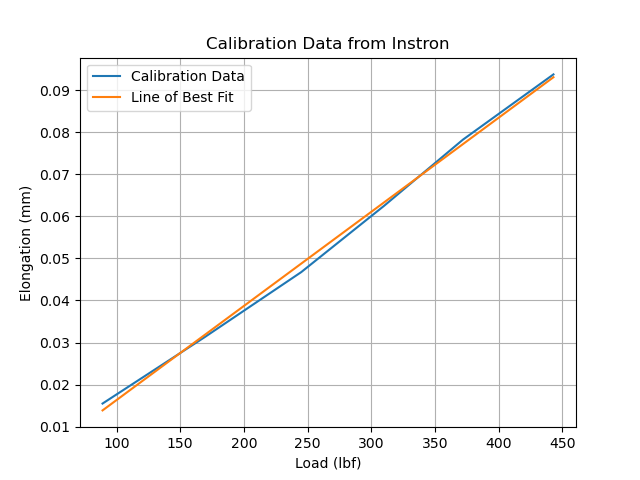
\includegraphics[width=4in]{images/graphs/Calibration Data}
		\caption{Calibration data provided by the TA graphed with a line of best fit.}
		\label{fig:calibration_data}
	\end{figure}
	
	\item The code shown in Listing \ref{code:corrected_elongation} corrects the elongation values collected from the Instron machine.
	
	\begin{lstlisting}[label={code:corrected_elongation}, caption={The code used to correct the elongation values collected from the Instron machine during the tensile test.},language=Python]
# Import tensile test data (Instron)
tensile_test_data_instron = pd.read_csv("Lab 4 Tensile Data Instron.csv")

time = (tensile_test_data_instron["Time (s)"].to_numpy() * ureg.s) # [s]
tensile_load = (tensile_test_data_instron["Load (lbf)"].to_numpy()
                * ureg.lbf) # [lbf]
tensile_extension = (
    tensile_test_data_instron["Extension (in)"].to_numpy()
    * ureg.inch) # [in]
...
# Correct the tensile test data from the instron
corrected_tensile_extension = (
    tensile_extension
    - (a1 * tensile_load + b1)).to(ureg.inch) # [in]\end{lstlisting}
    
    \item To convert the corrected elongation values collected from the Instron machine for the tensile test and to convert the recorded loads to stresses, we used the code in Listing \ref{code:average_strain}.
    
    \begin{lstlisting}[label={code:average_strain}, caption={The code used to convert the corrected elongations values into strains and the recorded loads into stresses.},language=Python]
# Define constants
gage_length     = 11 * ureg.cm      # [cm]
b               = 2 * ureg.inch     # [in]
h               = 0.025 * ureg.inch # [in]
...
# Calculate strain from the tensile test data from the instron
tensile_strain_instron =
	(corrected_tensile_extension / gage_length).to(
    ureg.dimensionless) # []

# Calculate stress from the tensile test data from the Instron
tensile_stress = (tensile_load / (b * h)).to(ureg.psi) # [psi]

# Create line of best fit for stress-strain curve from the Instron
a2,b2 = np.polyfit(tensile_strain_instron.magnitude,
                   tensile_stress.magnitude, 1)
a2 *= ureg.psi / ureg.dimensionless # [psi/]
b2 *= ureg.psi # [psi]
...
# Plot the stress-strain curve from the Instron
plt.figure()
plt.plot(tensile_strain_instron.magnitude, tensile_stress.magnitude,
         label="Tensile Test Data")
plt.plot(tensile_strain_instron.magnitude,
         (a2 * tensile_strain_instron + b2).to(ureg.psi).magnitude,
         label="Line of Best Fit")
plt.legend()
plt.grid()
plt.xlabel("Strain (in/in)")
plt.ylabel("Stress (psi)")
plt.title("Stress vs Strain (Instron)")\end{lstlisting}

	This code generated the graph shown in Figure \ref{fig:stress_strain_instron}.
	
	\begin{figure}[htbp]
		\centering
		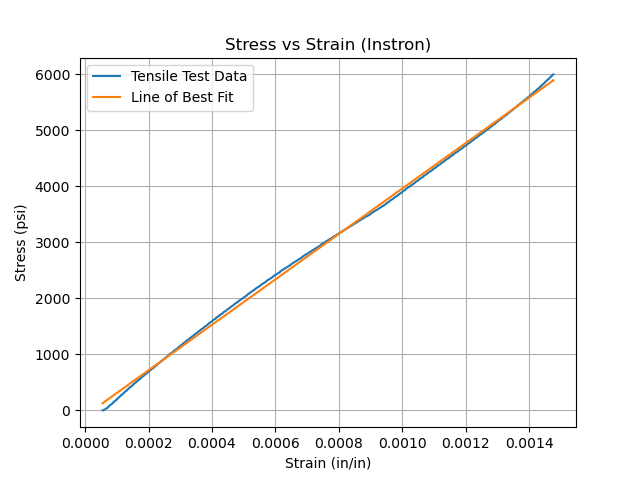
\includegraphics[width=4in]{images/graphs/Stress vs Strain Instron}
		\caption{The stress vs strain curve generated from the data recorded by the Instron machine during the tensile test.}
		\label{fig:stress_strain_instron}
	\end{figure}
	
	\item To plot the average strain calculated from the Instron machine with the strain measured by the yellow box, we used the code in Listing \ref{code:strains}
	
	\begin{lstlisting}[label={code:strains}, caption={The code used to plot the two strain measurements---one from the Instron machine and the other from the NI USB-6000---in the same graph.},language=Python]
# Smooth the tensile strain data from the yellow box
window = 15
smoothed_tensile_strain_yb = (
    np.convolve(tensile_strain_yb.magnitude, np.ones(window), "valid")
    / window * ureg.dimensionless) # []

# Get the time domain for the yellow box strain
time_yb = np.arange(time[0].magnitude, time[-1].magnitude,
                    (time[-1].magnitude - time[0].magnitude)
                    / len(smoothed_tensile_strain_yb)) * ureg.s # [s]
...
# Plot strain vs time
plt.figure()
plt.plot(time.magnitude, tensile_strain_instron.magnitude * 1e6,
         label="Tensile Strain (Instron)")
plt.plot(time_yb.magnitude, smoothed_tensile_strain_yb.magnitude * 1e6,
         label="Tensile Strain (Yellow Box)")
plt.legend()
plt.grid()
plt.xlabel("Time (s)")
plt.ylabel("Strain (microstrain)")
plt.title("Strain vs Time")\end{lstlisting}

	This code generated the graph shown in Figure \ref{fig:strains}
	
	\begin{figure}[htbp]
		\centering
		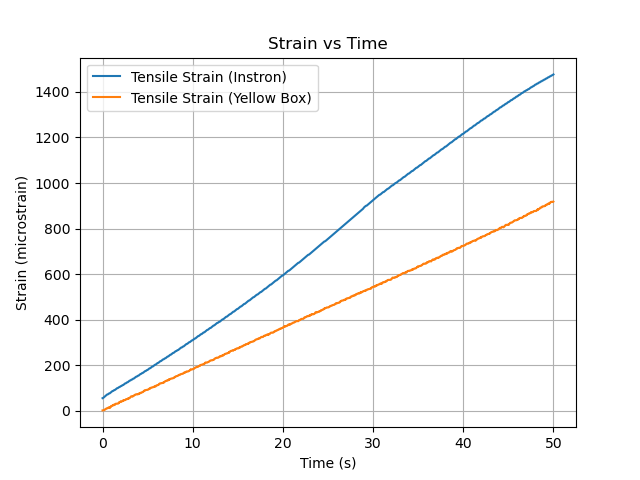
\includegraphics[width=4in]{images/graphs/Strain vs Time}
		\caption{The two strains, one measured from the Instron machine the other from the NI USB-6000, plotted over time.}
		\label{fig:strains}
	\end{figure}
	
	\item The average strain calculated by using the data from the Instron and the recorded strain from the NI USB-6000 (yellow box) vary significantly. The average error between the two strains was between \qtyrange{10}{20}{\%}. The variance could be accounted for in part by the fact that we could not get the calibration to work properly; we used data provided by the TA for calibration. Otherwise, we may have measured the gage length incorrectly.
	
	On the other hand, the strain gauges on our sample could have been damaged or setup improperly. Throughout the lab, we checked to ensure the strain gauges were zeroed appropriately, but if they were not centered, had too much solder, or were glued incorrectly, the strain values recorded by the NI USB-6000 would be inaccurate.
	
	It should be noted, however, that the difference between the two strain measurements was much greater as the test went on, \ie the stress increased. This leads us to believe that the calibration data we used could have had a significant impact on the strain calculated based on the Instron data.
	
	\item To plot the stress vs strain curve using the data from the NI USB-6000 (yellow box), we used the code shown in Listing \ref{code:stress_strain_yb}.
	
	\begin{lstlisting}[label={code:stress_strain_yb}, caption={The code used to plot the stress vs strain curve generated from the strain measurements taken by the NI USB-6000.},language=Python]
# Generate an equation for the stress
a3,b3 = np.polyfit(time.magnitude, tensile_stress.magnitude, 1)
a3 *= ureg.psi / ureg.s # [psi/s]
b3 *= ureg.psi # [psi]

# Calculate stress with respect to the yellow box strain
tensile_stress_yb = (a3 * time_yb + b3) # [psi]

# Calculate line of best fit for the yellow box stress-strain curve
a4,b4 = np.polyfit(smoothed_tensile_strain_yb.magnitude,
                   tensile_stress_yb.magnitude, 1)
a4 *= ureg.psi / ureg.dimensionless # [psi/]
b4 *= ureg.psi # [psi]
...
# Plot the stress-strain curve from the yellow box
plt.figure()
plt.plot(smoothed_tensile_strain_yb.magnitude,
         tensile_stress_yb.magnitude, label="Tensile Test Data")
plt.plot(smoothed_tensile_strain_yb.magnitude,
         (a4 * smoothed_tensile_strain_yb + b4).to(ureg.psi).magnitude,
         label="Line of Best Fit")
plt.legend()
plt.grid()
plt.xlabel("Strain (in/in)")
plt.ylabel("Stress (psi)")
plt.title("Stress vs Strain (Yellow Box)")\end{lstlisting}

	The plot generated by this code is shown in Figure \ref{fig:stress_strain_yb}.
	
	\begin{figure}[htbp]
		\centering
		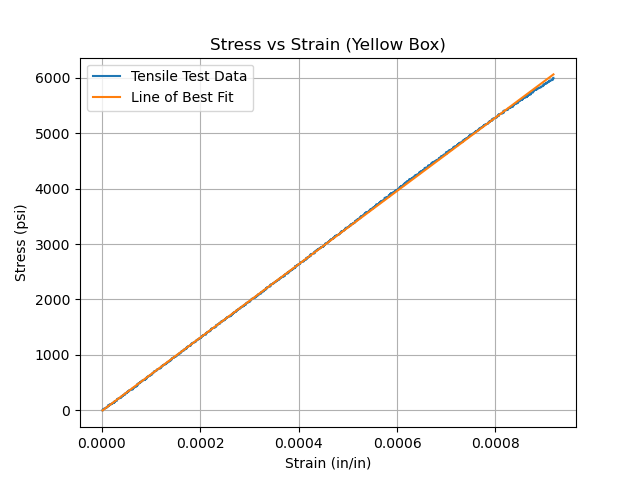
\includegraphics[width=4in]{images/graphs/Stress vs Strain YB}
		\caption{The stress vs strain curve generated by using strain measurements from the yellow box and stress measurements from the Instron machine.}
		\label{fig:stress_strain_yb}
	\end{figure}
	
	\item Since we already plotted lines of best fit for both stress--strain curves, finding the Young's Moduli for the respective graphs is trivial: the leading coefficients of the lines of best fit are the Young's Moduli. The code to calculate and plot these moduli is shown in Listing \ref{code:young}.
	
	\begin{lstlisting}[label={code:young}, caption={The code used to calculate and plot the Young's Moduli of the two stress--strain curves.},language=Python]
E_actual        = 73.1 * ureg.GPa   # [GPa]
...
# Calculate Young's Modulus
E_instron = a2.to(ureg.GPa) # [GPa]
E_yb = a4.to(ureg.GPa) # [GPa]
...
print("Young's Modulus (Actual)     = {:.2f}".format(E_actual))
print("Young's Modulus (Instron)    = {:.2f}".format(E_instron))
print("Young's Modulus (Yellow Box) = {:.2f}".format(E_yb))
...
# Plot the Young's Moduli
plt.figure()
plt.bar(["Actual", "Instron", "Yellow Box"],
        [E_actual.magnitude, E_instron.magnitude, E_yb.magnitude])
plt.xlabel("Young's Modulus")
plt.ylabel("GPa")
plt.title("Young's Modulus Comparison")
plt.show()\end{lstlisting}
\end{parlist}

	The plot generated by this code is shown in Figure \ref{fig:young}.
	
	\begin{figure}[htbp]
		\centering
		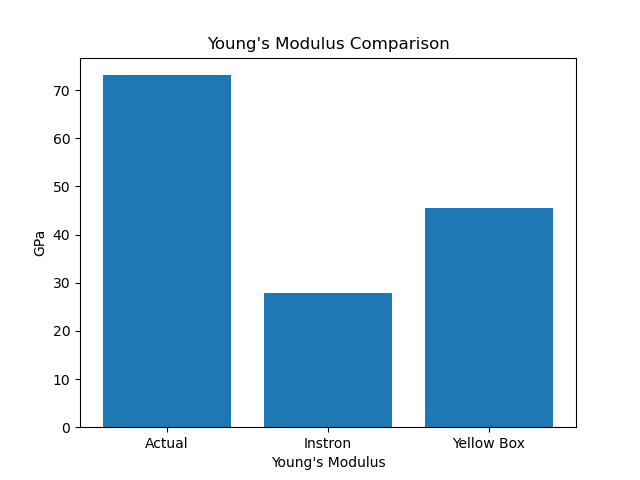
\includegraphics[width=4in]{images/graphs/Youngs Moduli}
		\caption{The Young's Moduli of the different stress--strain curves.}
		\label{fig:young}
	\end{figure}
	
	These values for $E$ are significantly less than the actual value of $E$ for the aluminum sample used. This is likely due to the same sources of error discussed in part (ix) of this analysis.

\section{Conclusion} \label{sec:conclusion}
Although our data did not match well with the theoretical values we expected, our code did successfully generate stress-strain curves and show how to record strain in different configurations.

\printbibliography[heading=subbibintoc]
\appendix
\chapter{Code} \label{ch:code}
\section{Lab\_4\_Analysis.py} \label{sec:lab_4_analysis.py}
\lstinputlisting[caption={Our data analysis script, \texttt{Lab\_4\_Analysis.py}.},language=Python]{src/Lab_4_Analysis.py}

\begin{verbatim}
Young's Modulus (Actual)     = 73.10 gigapascal
Young's Modulus (Instron)    = 27.96 gigapascal
Young's Modulus (Yellow Box) = 45.62 gigapascal
\end{verbatim}

\end{document}
